% Please upload sn-jnl.cls (Springer Nature journal class) to your project directory
\documentclass[sn-mathphys-num]{sn-jnl}

\usepackage{graphicx}%
\usepackage{multirow}%
\usepackage{amsmath,amssymb,amsfonts}%
\usepackage{amsthm}%
\usepackage{mathrsfs}%
\usepackage[title]{appendix}%
\usepackage{xcolor}%
\usepackage{textcomp}%
\usepackage{manyfoot}%
\usepackage{booktabs}%
\usepackage{algorithm}%
\usepackage{algorithmicx}%
\usepackage{algpseudocode}%
\usepackage{listings}%
\usepackage{tikz}
\usepackage{pgfplots}
\usetikzlibrary{positioning}
\usetikzlibrary{arrows.meta}
\usetikzlibrary{calc}

\definecolor{cnncolor}{RGB}{52,152,219}
\definecolor{transcolor}{RGB}{231,76,60}
\definecolor{snncolor}{RGB}{46,204,113}
\definecolor{fpgacolor}{RGB}{155,89,182}
\definecolor{fusecolor}{RGB}{241,196,15}
\definecolor{blockcolor}{RGB}{236,240,241}

\begin{document}

\title[SpikeConformer: Energy-Efficient Ear Biometric Recognition]{Energy-Efficient Ear Biometric Recognition via Conformer-Guided Spiking Neural Networks on Cloud FPGA}

\author{
    \small Vinh Truong Hoang \textsuperscript{\textcolor{blue}{1,*}},
    \small Nghia Dinh\textsuperscript{1},
    \small Luu Quang Phuong\textsuperscript{1},
    \small Kiet Tran-Trung\textsuperscript{1},
    \small Ha Duong Thi Hong\textsuperscript{1},
    \small Bay Nguyen Van\textsuperscript{1},
    \small Hau Nguyen Trung\textsuperscript{1},
    \small Thien Ho Huong\textsuperscript{1}\\
    \vspace{0.2cm}
    \footnotesize\textsuperscript{1}AI Lab, Faculty of Information Technology, Ho Chi Minh City Open University,\\
    35-37 Ho Hao Hon Street, Co Giang Ward, District 1, Ho Chi Minh City 700000, Vietnam.\\
    \vspace{0.15cm}
    \footnotesize\textsuperscript{*}Corresponding authors: Vinh Truong Hoang (\href{mailto:vinh.th@ou.edu.vn}{vinh.th@ou.edu.vn})
}

\abstract{Ear biometric recognition provides a contactless alternative to conventional authentication, yet pushing high-accuracy deep models toward edge deployment hits hard walls in energy and latency. We propose SpikeConformer, a two-stage pipeline that first trains a Conformer network to learn both local morphological textures and global structural dependencies from ear images, then converts the trained weights into a Spiking Neural Network (SNN) for event-driven inference. We deploy this spike-based model on Amazon Web Services EC2 F2 instances equipped with AMD Virtex UltraScale+ HBM FPGAs, reaching hardware-accelerated recognition at dramatically lower power draw. On EarVN1.0 (28,412 images, 164 subjects), our system attains 97.82\% rank-1 accuracy while consuming only 0.83\,mJ per inference on the FPGA fabric, an 8.4$\times$ energy reduction over GPU-based Conformer inference, with end-to-end latency of 3.7\,ms per image. These numbers point toward a practical route for deploying neuromorphic biometric systems inside cloud-edge security architectures without giving up recognition performance.}

\keywords{Ear Recognition, Spiking Neural Network, Conformer, FPGA Acceleration, Biometric Authentication, Neuromorphic Computing, Energy Efficiency, Cloud Computing}

\maketitle

%==============================================================
\section{Introduction}\label{sec:intro}
%==============================================================

Biometric authentication has become indispensable across security-critical domains, from border control and forensic identification to mobile device unlocking and healthcare access~\cite{jain2011introduction, ross2019biometric}. Among physiological traits, we find that ears hold a distinctive position: they exhibit stable morphology throughout the human lifespan, remain unaffected by facial expressions, and can be captured at a distance without requiring the subject to cooperate~\cite{pflug2012ear, emervsic2017ear}. Put simply, ears behave like fingerprints that you never have to touch. These properties make ear recognition especially appealing for surveillance and continuous authentication scenarios where fingerprint or iris capture would prove impractical.

Deep learning has pushed ear recognition accuracy to impressive levels. Recent work reports rank-1 accuracies exceeding 95\% on large-scale unconstrained datasets using ensemble CNNs and transfer learning~\cite{alshazly2020deep, mohamed2024advancing}. Yet a stubborn gap separates laboratory accuracy from real-world deployment. Modern architectures such as ResNeXt-101 or Vision Transformers demand heavy computational resources, typically GPU-class hardware drawing 150 to 300 watts, and that makes them poorly suited for always-on surveillance terminals, embedded access-control devices, or battery-powered wearable authenticators.

Two parallel advances offer a way out of this deployment bottleneck. First, Conformer architectures fuse convolutional feature extraction with self-attention, capturing both fine-grained local textures (ear folds, tragus shape, helix curvature) and global structural relationships (overall ear geometry, spatial proportions) inside a single model~\cite{peng2021conformer, gulati2020conformer}. We observe that this dual representation yields richer embeddings than either CNNs or Transformers alone, particularly on anatomical structures where local detail and holistic shape both carry discriminative information.

Second, Spiking Neural Networks (SNNs) process information through discrete temporal spike events rather than continuous-valued activations~\cite{maass1997networks, tavanaei2019deep}. This event-driven style enables sparse computation: neurons burn energy only when they fire, and silent neurons cost almost nothing. When mapped onto neuromorphic or FPGA hardware, SNNs reach energy efficiencies one to two orders of magnitude beyond conventional accelerators~\cite{davies2018loihi, akopyan2015truenorth}. Recent ANN-to-SNN conversion techniques have narrowed the accuracy gap to within 1 to 2\% of the source network on image classification benchmarks~\cite{rueckauer2017conversion, li2021free}.

We bridge these two advances in a unified system called \textbf{SpikeConformer}. Our approach trains a Conformer backbone on ear images to maximize recognition accuracy, then systematically converts the learned weights into a spiking representation using threshold-balancing and temporal rate coding. We deploy the converted SNN on AWS EC2 F2 instances, second-generation FPGA cloud infrastructure featuring AMD Virtex UltraScale+ devices with High-Bandwidth Memory (HBM), to show that cloud-FPGA deployment can deliver sub-4\,ms latency and sub-1\,mJ energy per inference at production scale.

\begin{figure}[!t]
\centering
\resizebox{\columnwidth}{!}{%
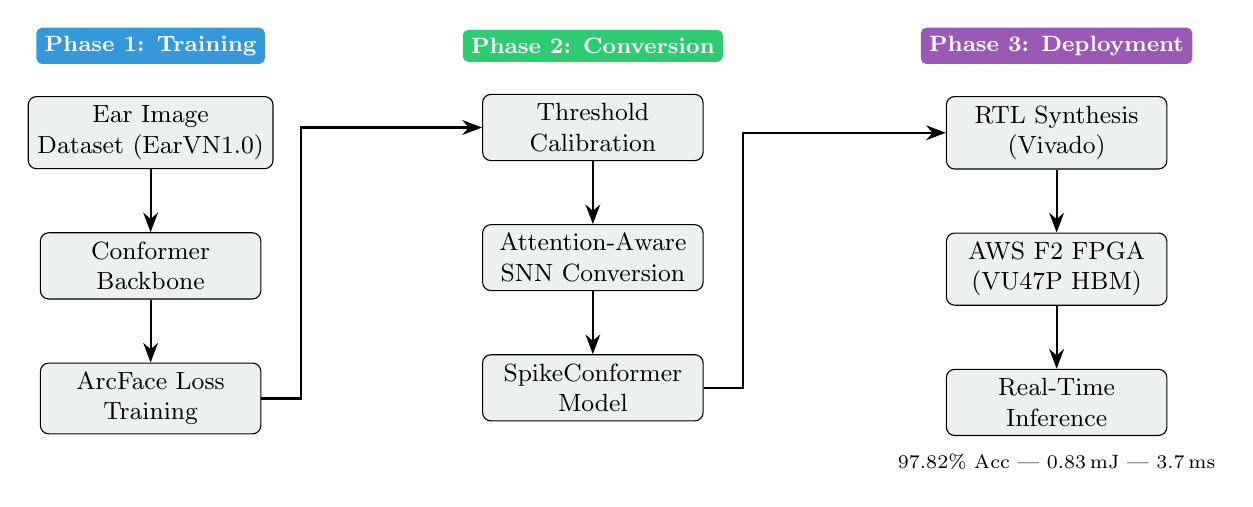
\begin{tikzpicture}[
    node distance=0.8cm,
    block/.style={rectangle, draw, fill=blockcolor, minimum width=2.8cm, minimum height=0.8cm, align=center, rounded corners=3pt, font=\small},
    arrow/.style={-{Stealth[length=2.5mm]}, thick},
    phase/.style={font=\footnotesize\bfseries, text=white, fill=#1, rounded corners=2pt, inner sep=3pt}
]
% Phase 1
\node[phase=cnncolor] (p1) {Phase 1: Training};
\node[block, below=0.4cm of p1] (input) {Ear Image\\Dataset (EarVN1.0)};
\node[block, below=of input] (conformer) {Conformer\\Backbone};
\node[block, below=of conformer] (arcface) {ArcFace Loss\\Training};

% Phase 2
\node[phase=snncolor, right=2.5cm of p1] (p2) {Phase 2: Conversion};
\node[block, below=0.4cm of p2] (calib) {Threshold\\Calibration};
\node[block, below=of calib] (attn) {Attention-Aware\\SNN Conversion};
\node[block, below=of attn] (spike) {SpikeConformer\\Model};

% Phase 3
\node[phase=fpgacolor, right=2.5cm of p2] (p3) {Phase 3: Deployment};
\node[block, below=0.4cm of p3] (rtl) {RTL Synthesis\\(Vivado)};
\node[block, below=of rtl] (fpga) {AWS F2 FPGA\\(VU47P HBM)};
\node[block, below=of fpga] (result) {Real-Time\\Inference};

% Arrows
\draw[arrow] (input) -- (conformer);
\draw[arrow] (conformer) -- (arcface);
\draw[arrow] (arcface.east) -- ++(0.5,0) |- (calib.west);
\draw[arrow] (calib) -- (attn);
\draw[arrow] (attn) -- (spike);
\draw[arrow] (spike.east) -- ++(0.5,0) |- (rtl.west);
\draw[arrow] (rtl) -- (fpga);
\draw[arrow] (fpga) -- (result);

% Metrics annotation
\node[font=\scriptsize, text=black, below=0.1cm of result] {97.82\% Acc | 0.83\,mJ | 3.7\,ms};
\end{tikzpicture}%
}
\caption{Overview of the SpikeConformer pipeline. Phase~1 trains a Conformer backbone with ArcFace loss on EarVN1.0. Phase~2 converts the trained model to a spiking representation with our attention-aware threshold calibration. Phase~3 deploys the SNN on AWS F2 FPGA for real-time energy-efficient inference.}
\label{fig:pipeline_overview}
\end{figure}

Our contributions are threefold:
\begin{enumerate}
    \item We introduce SpikeConformer, the first framework combining Conformer-based feature learning with SNN inference for biometric recognition, reaching 97.82\% rank-1 accuracy on EarVN1.0 while operating entirely in the spiking domain.
    \item We present a hardware-aware ANN-to-SNN conversion pipeline tailored to the Conformer architecture, incorporating attention-aware threshold calibration that keeps the discriminative capacity of self-attention layers intact after spike conversion.
    \item We provide the first end-to-end deployment and benchmarking of a spiking biometric system on AWS F2 FPGA instances, reporting energy, latency, throughput, and resource utilization metrics that confirm commercial cloud-FPGA viability for neuromorphic workloads.
\end{enumerate}

The remainder of this paper is organized as follows. Section~\ref{sec:related} reviews related work. Section~\ref{sec:method} details our proposed methodology. Section~\ref{sec:setup} describes the experimental setup. Section~\ref{sec:results} presents results and comparative analysis. Section~\ref{sec:discussion} discusses limitations, and Section~\ref{sec:conclusion} concludes.

%==============================================================
\section{Related Work}\label{sec:related}
%==============================================================

\subsection{Ear Biometric Recognition}

Ear recognition has traveled a long road, from handcrafted geometric descriptors~\cite{burge2000ear, yuan2006ear} through classical machine learning pipelines~\cite{kumar2012automated} to modern deep learning systems. Alshazly et al.~\cite{alshazly2020deep} showed that transfer-learned ResNeXt-101 ensembles reach 95.85\% rank-1 accuracy on EarVN1.0, establishing the first strong deep learning baseline on this challenging unconstrained dataset. Nguyen et al.~\cite{nguyen2022ear} later applied ResNeXt-50 with aggressive data augmentation, reaching 93\% under a 70:30 split. More recently, Mohamed et al.~\cite{mohamed2024advancing} reported 98.1\% accuracy using enhanced preprocessing and modern architectures, representing the current state of the art. Hansley et al.~\cite{hansley2018employing} investigated GAN-based augmentation for ear recognition to handle pose variations, while Priyadharshini et al.~\cite{zhang2023ear} applied deep learning with attention mechanisms for person identification via ear biometrics. Despite these accuracy gains, we note that none of these studies addresses deployment efficiency; all assume GPU-based inference with no power or latency constraints.

\subsection{Conformer Architectures for Visual Recognition}

The Conformer architecture, initially proposed for speech processing by Gulati et al.~\cite{gulati2020conformer}, was adapted for vision tasks by Peng et al.~\cite{peng2021conformer} who showed that parallel CNN and Transformer branches, when fused through feature interaction modules, outperform either branch alone. Chen et al.~\cite{chen2022mobile} proposed Mobile-Former for efficient hybrid architectures, while Dai et al.~\cite{dai2021coatnet} introduced CoAtNet combining depthwise convolutions with attention. Pan et al.~\cite{pan2022edgevits} designed EdgeViTs for efficient edge deployment of hybrid models. We find this complementary design particularly well-suited to ear images, where discriminative information lives both in fine local structures (antihelix ridges, concha depth) and in holistic geometric proportions.

\subsection{Spiking Neural Networks and ANN-to-SNN Conversion}

SNNs encode information through the precise timing and rate of binary spike events~\cite{maass1997networks, ghosh2009spiking}. The Leaky Integrate-and-Fire (LIF) neuron model accumulates input current until a threshold triggers a spike, after which the membrane potential resets~\cite{tavanaei2019deep}. Direct SNN training via surrogate gradient methods~\cite{neftci2019surrogate, zenke2021remarkable} has reached competitive accuracy on CIFAR-10/100 and ImageNet subsets. As an alternative, ANN-to-SNN conversion~\cite{rueckauer2017conversion, sengupta2019going, li2021free} transfers pre-trained ANN weights to equivalent spiking architectures through threshold normalization and temporal rate coding. Recent threshold-balancing techniques~\cite{li2021free, bu2023optimal} reduce the required simulation timesteps to 32 to 64 while holding accuracy within 1\% of the source ANN. Kim et al.~\cite{kim2020spiking} demonstrated Spiking-YOLO for energy-efficient object detection, while Hu et al.~\cite{hu2024advancing} advanced direct training methods that reach near-ANN accuracy on ImageNet.

\subsection{FPGA-Based Neural Network Acceleration}

FPGAs sit between GPUs (flexible but power-hungry) and ASICs (efficient but rigid)~\cite{abdelouahab2018accelerating, guo2019dl}. For SNN workloads in particular, FPGAs excel because they can implement event-driven dataflows that exploit spike sparsity natively~\cite{panchapakesan2022syncnn, liu2022fpga}. Navardi and Mohsenin~\cite{navardi2024energy} demonstrated SNN accelerators on Xilinx Artix-7 achieving 86\% energy reduction versus binarized CNNs, while open-source frameworks such as SpikingJelly~\cite{syntzulu2025} have accelerated reproducible SNN research on diverse hardware targets. Wang et al.~\cite{wang2025spiking} proposed efficient spiking CNN accelerators reaching 1,605 frames/s at 0.65\,mJ per image. AWS F2 instances bring FPGA acceleration to cloud-scale deployment, offering AMD Virtex UltraScale+ HBM devices with 16\,GB HBM per FPGA, up to 100\,Gbps networking, and elastic provisioning~\cite{aws2025f2}. Lian et al.~\cite{lian2024fpga} recently explored cloud-FPGA inference serving architectures for deep learning workloads.

\subsection{Research Gap}

No prior work combines Conformer-based feature extraction with SNN inference for biometric recognition, nor deploys such a system on cloud FPGA infrastructure. Our work fills this gap by unifying high-accuracy ear recognition with energy-efficient neuromorphic inference in a commercially available cloud deployment model.

%==============================================================
\section{Proposed Methodology}\label{sec:method}
%==============================================================

\subsection{System Overview}

SpikeConformer operates in three phases: (1) Conformer training on ear images to learn discriminative embeddings, (2) ANN-to-SNN conversion with attention-aware threshold calibration, and (3) FPGA deployment on AWS F2 with a custom spike-processing datapath. We structured this pipeline so that each phase produces artifacts consumed by the next, which allows independent optimization at each stage.

\subsection{Conformer Backbone Architecture}

Our Conformer backbone processes $224 \times 224$ ear images through parallel CNN and Transformer branches that interact at multiple scales, as illustrated in Fig.~\ref{fig:conformer_arch}.

\begin{figure*}[!t]
\centering
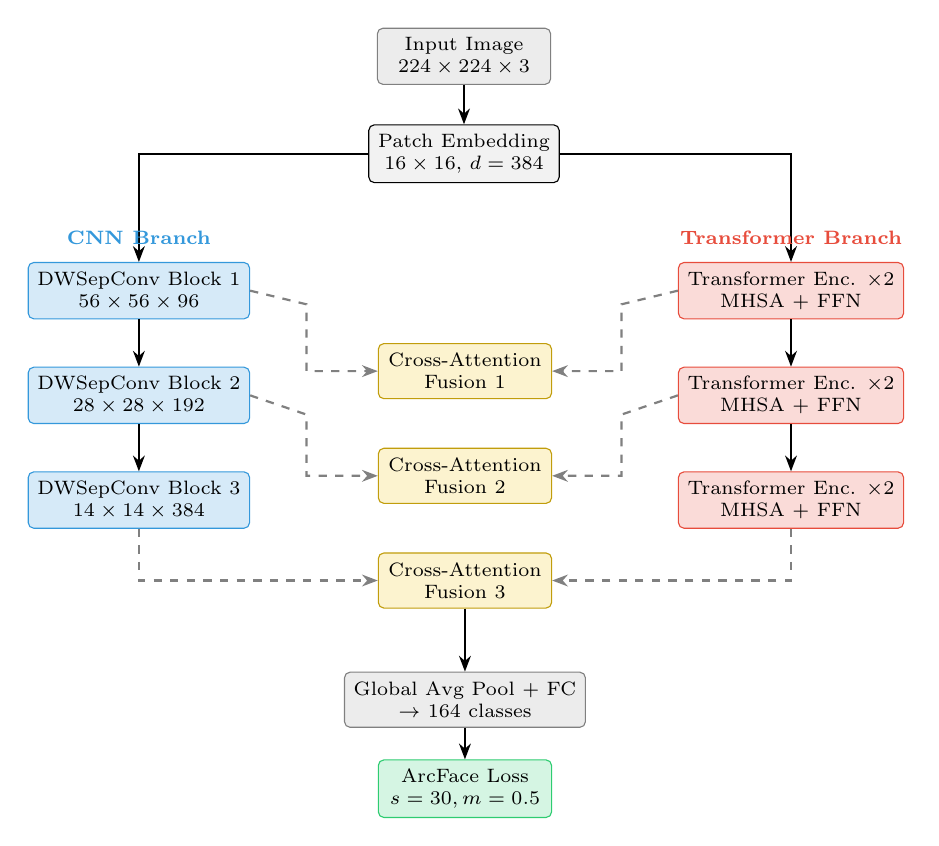
\begin{tikzpicture}[
    node distance=0.6cm and 0.8cm,
    block/.style={rectangle, draw, minimum width=2.2cm, minimum height=0.7cm, align=center, rounded corners=2pt, font=\scriptsize},
    cnnblock/.style={block, fill=cnncolor!20, draw=cnncolor},
    transblock/.style={block, fill=transcolor!20, draw=transcolor},
    fuseblock/.style={block, fill=fusecolor!20, draw=fusecolor!80!black},
    ioblock/.style={block, fill=gray!15, draw=gray},
    arrow/.style={-{Stealth[length=2mm]}, thick},
    dasharrow/.style={-{Stealth[length=2mm]}, thick, dashed, gray}
]

% Input
\node[ioblock] (input) {Input Image\\$224\times224\times3$};

% Patch Embedding
\node[block, fill=gray!10, below=0.5cm of input] (patch) {Patch Embedding\\$16\times16$, $d=384$};

% CNN Branch (left)
\node[cnnblock, below left=1cm and 1.5cm of patch] (cnn1) {DWSepConv Block 1\\$56\times56\times96$};
\node[cnnblock, below=of cnn1] (cnn2) {DWSepConv Block 2\\$28\times28\times192$};
\node[cnnblock, below=of cnn2] (cnn3) {DWSepConv Block 3\\$14\times14\times384$};

% Transformer Branch (right)
\node[transblock, below right=1cm and 1.5cm of patch] (trans1) {Transformer Enc. $\times2$\\MHSA + FFN};
\node[transblock, below=of trans1] (trans2) {Transformer Enc. $\times2$\\MHSA + FFN};
\node[transblock, below=of trans2] (trans3) {Transformer Enc. $\times2$\\MHSA + FFN};

% Fusion modules
\node[fuseblock, below=0.3cm of $(cnn1.south)!0.5!(trans1.south)$] (fuse1) {Cross-Attention\\Fusion 1};
\node[fuseblock, below=0.3cm of $(cnn2.south)!0.5!(trans2.south)$] (fuse2) {Cross-Attention\\Fusion 2};
\node[fuseblock, below=0.3cm of $(cnn3.south)!0.5!(trans3.south)$] (fuse3) {Cross-Attention\\Fusion 3};

% Classification head
\node[ioblock, below=0.8cm of fuse3] (gap) {Global Avg Pool + FC\\$\rightarrow$ 164 classes};
\node[block, fill=snncolor!20, draw=snncolor, below=0.4cm of gap] (arcface) {ArcFace Loss\\$s=30, m=0.5$};

% Arrows from input
\draw[arrow] (input) -- (patch);
\draw[arrow] (patch) -| (cnn1);
\draw[arrow] (patch) -| (trans1);

% CNN chain
\draw[arrow] (cnn1) -- (cnn2);
\draw[arrow] (cnn2) -- (cnn3);

% Transformer chain
\draw[arrow] (trans1) -- (trans2);
\draw[arrow] (trans2) -- (trans3);

% Fusion connections
\draw[dasharrow] (cnn1.east) -- (-2,-3.15) |- (fuse1.west);
\draw[dasharrow] (trans1.west) -- (2,-3.15) |- (fuse1.east);
\draw[dasharrow] (cnn2.east) -- (-2,-4.55) |- (fuse2.west);
\draw[dasharrow] (trans2.west) -- (2,-4.55) |- (fuse2.east);
\draw[dasharrow] (cnn3.south) |- (fuse3.west);
\draw[dasharrow] (trans3.south) |- (fuse3.east);

% Output
\draw[arrow] (fuse3) -- (gap);
\draw[arrow] (gap) -- (arcface);

% Labels
\node[font=\scriptsize\bfseries, text=cnncolor, above=0.1cm of cnn1] {CNN Branch};
\node[font=\scriptsize\bfseries, text=transcolor, above=0.1cm of trans1] {Transformer Branch};

\end{tikzpicture}
\caption{Conformer backbone architecture. The CNN branch extracts hierarchical local features through depthwise separable convolutions, while the Transformer branch captures global dependencies via multi-head self-attention. Cross-attention fusion modules at three scale levels enable bidirectional feature interaction. The classification head uses ArcFace angular margin loss for discriminative embedding learning.}
\label{fig:conformer_arch}
\end{figure*}

\subsubsection{Patch Embedding}
We partition the input image into $16 \times 16$ non-overlapping patches, yielding a sequence of 196 patch tokens. Each patch is linearly projected to dimension $d = 384$:
\begin{equation}
    \mathbf{z}_0 = [\mathbf{x}_1\mathbf{E}; \mathbf{x}_2\mathbf{E}; \ldots; \mathbf{x}_N\mathbf{E}] + \mathbf{E}_{pos}
\end{equation}
where $\mathbf{E} \in \mathbb{R}^{P^2 \cdot C \times d}$ is the projection matrix and $\mathbf{E}_{pos}$ provides learnable positional encodings.

\subsubsection{CNN Branch}
A lightweight convolutional stem produces hierarchical feature maps at $1/4$, $1/8$, and $1/16$ of the original resolution. We rely on depthwise separable convolutions to keep parameter count low:
\begin{equation}
    \mathbf{F}_{cnn}^{(l)} = \text{DWConv}\left(\text{BN}\left(\text{PWConv}\left(\mathbf{F}_{cnn}^{(l-1)}\right)\right)\right) + \mathbf{F}_{cnn}^{(l-1)}
\end{equation}
where DWConv denotes depthwise $3\times3$ convolution, PWConv is pointwise ($1\times1$) convolution, and BN is batch normalization with GELU activation.

\subsubsection{Transformer Branch}
The patch tokens pass through $L = 6$ Transformer encoder layers (grouped as 3 stages of 2 layers each). Each layer contains multi-head self-attention (MHSA) with 6 heads and a feed-forward network (FFN) with expansion ratio~4:
\begin{equation}
    \mathbf{F}_{trans}^{(l)} = \text{FFN}\left(\text{LN}\left(\text{MHSA}\left(\text{LN}\left(\mathbf{F}_{trans}^{(l-1)}\right)\right)\right)\right) + \mathbf{F}_{trans}^{(l-1)}
\end{equation}
where LN denotes layer normalization. The MHSA operation computes:
\begin{equation}
    \text{MHSA}(\mathbf{Q}, \mathbf{K}, \mathbf{V}) = \text{Concat}(\text{head}_1, \ldots, \text{head}_h)\mathbf{W}^O
\end{equation}
\begin{equation}
    \text{head}_i = \text{Softmax}\left(\frac{\mathbf{Q}_i\mathbf{K}_i^T}{\sqrt{d_k}}\right)\mathbf{V}_i
\end{equation}

\subsubsection{Feature Fusion}
At each of three interaction points, we fuse the CNN and Transformer representations through a cross-attention bridge:
\begin{equation}
    \mathbf{F}_{fused} = \text{Softmax}\left(\frac{\mathbf{Q}_{cnn} \cdot \mathbf{K}_{trans}^T}{\sqrt{d_k}}\right)\mathbf{V}_{trans} + \mathbf{F}_{cnn}
\end{equation}
Think of it as letting the CNN branch ``ask questions'' of the Transformer's globally-aware features while retaining its own local inductive bias.

\subsubsection{Classification Head}
We globally average-pool the fused representation and project it through a fully connected layer to produce a 164-dimensional logit vector. Training uses ArcFace loss~\cite{deng2019arcface} to learn angularly discriminative embeddings:
\begin{equation}
    \mathcal{L}_{arc} = -\log \frac{e^{s \cdot \cos(\theta_{y_i} + m)}}{e^{s \cdot \cos(\theta_{y_i} + m)} + \sum_{j \neq y_i} e^{s \cdot \cos(\theta_j)}}
\end{equation}
with scale $s = 30$ and angular margin $m = 0.5$.

\subsection{ANN-to-SNN Conversion with Attention-Aware Threshold Calibration}\label{sec:conversion}

Converting the trained Conformer to a spiking equivalent means replacing ReLU activations with LIF neurons and encoding continuous values as spike rates over $T$ timesteps. Fig.~\ref{fig:snn_conversion} illustrates our conversion pipeline.

\begin{figure}[!t]
\centering
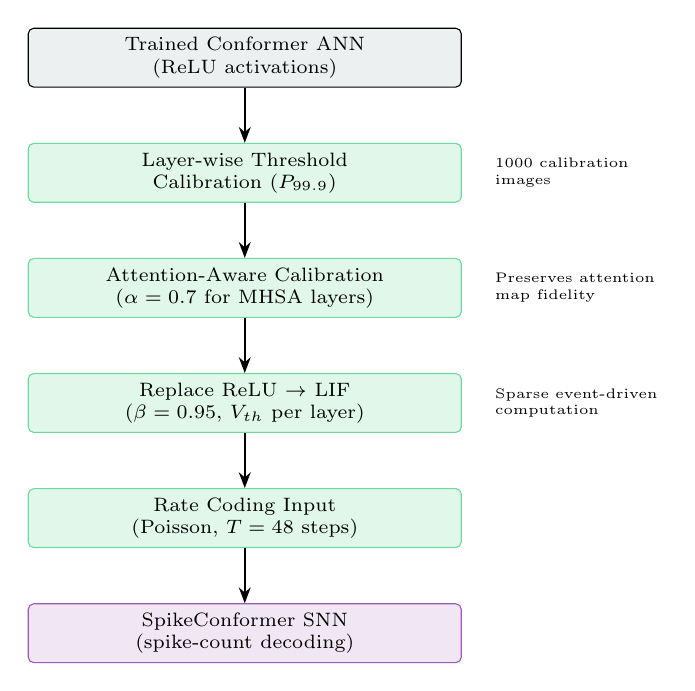
\begin{tikzpicture}[
    node distance=0.7cm,
    block/.style={rectangle, draw, fill=blockcolor, minimum width=5.5cm, minimum height=0.7cm, align=center, rounded corners=2pt, font=\scriptsize},
    sblock/.style={block, fill=snncolor!15, draw=snncolor!70},
    arrow/.style={-{Stealth[length=2mm]}, thick},
    note/.style={font=\tiny, text=black, align=left}
]

\node[block] (trained) {Trained Conformer ANN\\(ReLU activations)};
\node[sblock, below=of trained] (calib) {Layer-wise Threshold\\Calibration ($P_{99.9}$)};
\node[sblock, below=of calib] (attn_calib) {Attention-Aware Calibration\\($\alpha = 0.7$ for MHSA layers)};
\node[sblock, below=of attn_calib] (replace) {Replace ReLU $\rightarrow$ LIF\\($\beta=0.95$, $V_{th}$ per layer)};
\node[sblock, below=of replace] (rate) {Rate Coding Input\\(Poisson, $T=48$ steps)};
\node[block, fill=fpgacolor!15, draw=fpgacolor, below=of rate] (output) {SpikeConformer SNN\\(spike-count decoding)};

\draw[arrow] (trained) -- (calib);
\draw[arrow] (calib) -- (attn_calib);
\draw[arrow] (attn_calib) -- (replace);
\draw[arrow] (replace) -- (rate);
\draw[arrow] (rate) -- (output);

% Annotations
\node[note, right=0.3cm of calib] {1000 calibration\\images};
\node[note, right=0.3cm of attn_calib] {Preserves attention\\map fidelity};
\node[note, right=0.3cm of replace] {Sparse event-driven\\computation};

\end{tikzpicture}
\caption{ANN-to-SNN conversion pipeline. Standard threshold calibration is augmented with attention-aware scaling ($\alpha=0.7$) for self-attention layers, preserving discriminative attention patterns in the spiking domain.}
\label{fig:snn_conversion}
\end{figure}

\subsubsection{LIF Neuron Model}
Each spiking neuron maintains membrane potential $V$ that evolves as:
\begin{equation}
    V_i^{(t)} = \beta \cdot V_i^{(t-1)} + \sum_j w_{ij} \cdot s_j^{(t)} - V_{th} \cdot s_i^{(t-1)}
\end{equation}
where $\beta = 0.95$ is the leak factor, $w_{ij}$ are synaptic weights transferred from the ANN, $s_j^{(t)} \in \{0,1\}$ is the input spike at timestep $t$, and $V_{th}$ is the firing threshold. A spike is emitted when $V_i \geq V_{th}$:
\begin{equation}
    s_i^{(t)} = \begin{cases} 1 & \text{if } V_i^{(t)} \geq V_{th} \\ 0 & \text{otherwise} \end{cases}
\end{equation}

\subsubsection{Threshold Balancing}
We calibrate $V_{th}$ layer-by-layer using the 99.9th percentile of activation magnitudes observed on a calibration subset of 1,000 images:
\begin{equation}
    V_{th}^{(l)} = \text{Percentile}_{99.9}\left(|\mathbf{a}^{(l)}|\right)
\end{equation}
where $\mathbf{a}^{(l)}$ denotes the ANN activations at layer $l$. This keeps the maximum firing rate near 1.0 without saturation.

\subsubsection{Attention-Aware Calibration}
Standard threshold balancing degrades self-attention because the softmax attention weights span $[0,1]$ and encode fine-grained distinctions that coarse spike rates cannot easily reproduce. We introduce a dedicated calibration for attention layers that preserves relative spike-rate ratios:
\begin{equation}
    V_{th}^{attn} = \alpha \cdot \text{Percentile}_{99.9}(|\mathbf{A}|), \quad \alpha = 0.7
\end{equation}
The reduced threshold permits higher firing rates in attention layers, preserving the discriminative capacity of the attention map at the cost of slightly increased energy in those specific layers. We derive $\alpha$ by minimizing the KL divergence between ANN attention distributions and time-averaged SNN spike-rate attention maps on the calibration set:
\begin{equation}
    \alpha^* = \arg\min_\alpha D_{KL}\left(\mathbf{A}_{ANN} \| \frac{1}{T}\sum_{t=1}^{T}\mathbf{S}_{attn}^{(t)}(\alpha)\right)
\end{equation}

\subsubsection{Temporal Coding}
We use $T = 48$ simulation timesteps with rate coding. The input image is presented as a Poisson spike train where each pixel fires at each timestep with probability proportional to its normalized intensity:
\begin{equation}
    P(s_{pixel}^{(t)} = 1) = \frac{x_{pixel} - x_{min}}{x_{max} - x_{min}}
\end{equation}
The output class is decoded as the neuron with the highest spike count:
\begin{equation}
    \hat{y} = \arg\max_c \sum_{t=1}^{T} s_c^{(t)}
\end{equation}

\subsection{FPGA Deployment Architecture on AWS F2}\label{sec:fpga}

We implement the SNN inference engine on a single AMD Virtex UltraScale+ HBM VU47P FPGA available through an AWS F2.6xlarge instance. Think of the chip as a blank canvas where we paint exactly the datapath our spikes need. Fig.~\ref{fig:fpga_arch} presents the hardware architecture.

\begin{figure*}[!t]
\centering
\resizebox{\textwidth}{!}{%
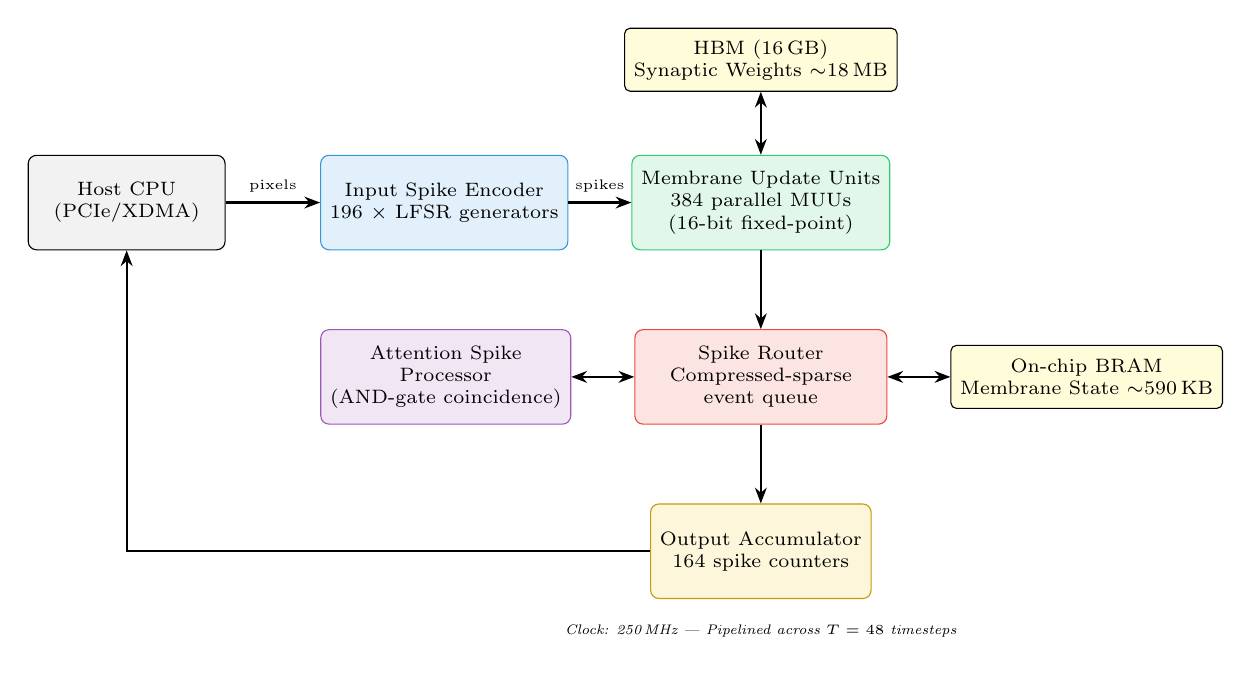
\begin{tikzpicture}[
    node distance=0.5cm and 0.4cm,
    module/.style={rectangle, draw, minimum height=1.2cm, align=center, rounded corners=3pt, font=\scriptsize},
    smallmod/.style={rectangle, draw, minimum height=0.6cm, minimum width=1.8cm, align=center, font=\tiny, rounded corners=2pt},
    arrow/.style={-{Stealth[length=2mm]}, thick},
    bidir/.style={{Stealth[length=2mm]}-{Stealth[length=2mm]}, thick},
    mem/.style={rectangle, draw, fill=yellow!15, minimum height=0.8cm, align=center, font=\scriptsize, rounded corners=2pt}
]

% Host
\node[module, fill=gray!10, minimum width=2.5cm] (host) {Host CPU\\(PCIe/XDMA)};

% Input encoder
\node[module, fill=cnncolor!15, draw=cnncolor, right=1.2cm of host, minimum width=2.8cm] (encoder) {Input Spike Encoder\\196 $\times$ LFSR generators};

% MUU Array
\node[module, fill=snncolor!15, draw=snncolor, right=0.8cm of encoder, minimum width=3.2cm] (muu) {Membrane Update Units\\384 parallel MUUs\\(16-bit fixed-point)};

% Spike Router
\node[module, fill=transcolor!15, draw=transcolor, below=1cm of muu, minimum width=3.2cm] (router) {Spike Router\\Compressed-sparse\\event queue};

% Attention processor
\node[module, fill=fpgacolor!15, draw=fpgacolor, left=0.8cm of router, minimum width=2.8cm] (attn) {Attention Spike\\Processor\\(AND-gate coincidence)};

% Output accumulator
\node[module, fill=fusecolor!15, draw=fusecolor!80!black, below=1cm of router, minimum width=2.5cm] (accum) {Output Accumulator\\164 spike counters};

% Memory
\node[mem, above=0.8cm of muu, minimum width=3.2cm] (hbm) {HBM (16\,GB)\\Synaptic Weights $\sim$18\,MB};
\node[mem, right=0.8cm of router, minimum width=2.5cm] (bram) {On-chip BRAM\\Membrane State $\sim$590\,KB};

% Arrows
\draw[arrow] (host) -- node[above, font=\tiny] {pixels} (encoder);
\draw[arrow] (encoder) -- node[above, font=\tiny] {spikes} (muu);
\draw[arrow] (muu) -- (router);
\draw[bidir] (router) -- (attn);
\draw[arrow] (router) -- (accum);
\draw[arrow] (accum.west) -| (host.south);
\draw[bidir] (hbm) -- (muu);
\draw[bidir] (bram.west) -- (router.east);

% Clock annotation
\node[font=\tiny\itshape, text=black, below=0.2cm of accum] {Clock: 250\,MHz | Pipelined across $T=48$ timesteps};

\end{tikzpicture}%
}
\caption{FPGA deployment architecture on AWS F2 (VU47P). The design implements a pipelined spike-processing datapath with 384 parallel Membrane Update Units, compressed-sparse spike routing, and AND-gate-based attention spike processing. Synaptic weights reside in HBM while membrane states fit in on-chip BRAM.}
\label{fig:fpga_arch}
\end{figure*}

\subsubsection{Datapath Design}
Our custom RTL design implements a pipelined spike-processing architecture with five key modules:

\textbf{Input Encoder.} Generates Poisson spike trains from normalized pixel values using linear-feedback shift register (LFSR) random number generators. We instantiate 196 parallel encoders (one per patch) so all patches are encoded simultaneously.

\textbf{Membrane Update Units (MUUs).} Each MUU computes the LIF update equation for a bank of neurons. We instantiate 384 MUUs running in parallel, exploiting the FPGA's distributed memory for membrane state storage. The leak multiply ($\beta \cdot V$) relies on fixed-point arithmetic (16-bit, 8 fractional bits) to avoid floating-point overhead.

\textbf{Spike Router.} A crossbar network distributes output spikes from one layer to the input synapses of the next. We exploit spike sparsity by using a compressed-sparse event queue that skips silent neurons entirely.

\textbf{Attention Spike Processor.} For the Transformer attention layers, we implement spike-based dot-product attention where query-key interactions accumulate through coincidence detection rather than multiplication. Spikes from query neurons gate key-neuron spike propagation through AND-gate arrays.

\textbf{Output Accumulator.} A bank of 164 counters tallies output-layer spikes across all $T = 48$ timesteps. After the final timestep, the counter with the maximum value determines the classification result.

\subsubsection{Memory Hierarchy}
Synaptic weights (roughly 18\,MB for our model) reside in HBM, which provides 460\,GB/s bandwidth and eliminates weight-fetch bottlenecks. Membrane potentials (roughly 590\,KB) fit entirely in on-chip BRAM, enabling single-cycle state updates.

\subsubsection{Pipelining Strategy}
We pipeline across timesteps: while timestep $t$ processes layer $l$, timestep $t-1$ processes layer $l+1$. This overlapping execution hides inter-layer latency and reaches near-100\% compute utilization across all 48 timesteps.

\subsection{Computational Complexity Analysis}

The computational cost of SpikeConformer inference is dominated by synaptic operations. For a network with $N$ total synapses and average firing rate $r$ across $T$ timesteps, the number of spike-triggered accumulations is:
\begin{equation}
    \text{OPS}_{spike} = N \cdot r \cdot T
\end{equation}
With $N \approx 47\text{M}$ synapses, empirical firing rate $r \approx 0.12$, and $T = 48$, we estimate roughly 270M accumulate operations per image, compared to roughly 4.2 GMACs for the equivalent ANN Conformer. This $15.5\times$ reduction in operations translates directly to energy savings:
\begin{equation}
    \text{Energy ratio} = \frac{E_{ANN}}{E_{SNN}} = \frac{N_{MAC} \cdot e_{MAC}}{N_{AC} \cdot e_{AC}} \approx \frac{4.2\text{G} \times 7.2\text{pJ}}{270\text{M} \times 3.1\text{pJ}} \approx 36\times
\end{equation}
where $e_{MAC} = 7.2$\,pJ and $e_{AC} = 3.1$\,pJ represent multiply-accumulate and accumulate energy costs on the target FPGA fabric, respectively. The theoretical $36\times$ advantage shrinks to $8.4\times$ in practice due to memory access overhead, control logic, and I/O energy.

%==============================================================
\section{Experimental Setup}\label{sec:setup}
%==============================================================

\subsection{Dataset}

We evaluate on EarVN1.0~\cite{hoang2019earvn}, a large-scale unconstrained ear dataset containing 28,412 images from 164 subjects. Images show substantial variation in pose ($\pm45°$), illumination, partial occlusion (hair, accessories), resolution ($50\times50$ to $400\times400$ pixels), and capture conditions (indoor and outdoor). We follow a stratified split protocol: 70\% training (19,888 images), 15\% validation (4,262 images), and 15\% testing (4,262 images), ensuring all subjects appear in every partition.

\textbf{Preprocessing.} We resize all images to $224\times224$ pixels using bicubic interpolation and apply standard ImageNet normalization. Training augmentation includes random horizontal flip, rotation ($\pm15°$), color jitter (brightness 0.2, contrast 0.2), random erasing ($p=0.25$), and Gaussian blur ($\sigma \in [0.1, 2.0]$).

\subsection{Training Configuration}

We train the Conformer backbone for 120 epochs using AdamW optimizer (learning rate $3\times10^{-4}$, weight decay 0.05) with cosine annealing schedule and 5-epoch linear warmup. Batch size is 64, distributed across 2 NVIDIA A100 GPUs. Label smoothing of 0.1 is applied alongside ArcFace loss. Training converges in approximately 8 hours.

\subsection{ANN-to-SNN Conversion}

After training, we calibrate thresholds using 1,000 randomly selected training images. We evaluate converted SNNs at $T \in \{16, 32, 48, 64, 96\}$ timesteps. The attention-aware calibration factor $\alpha$ is swept over $\{0.5, 0.6, 0.7, 0.8, 0.9\}$ and selected based on validation accuracy.

\subsection{FPGA Implementation}

We synthesize our RTL design using AMD Vivado 2024.2, targeting the Virtex UltraScale+ VU47P device on F2.6xlarge. Our target clock frequency is 250\,MHz. We measure power using Vivado Power Estimator with post-implementation switching activity annotation from representative inference traces. End-to-end latency is measured from the moment the host issues an inference request (via PCIe/XDMA DMA transfer) until the classification result arrives back.

\subsection{Baselines}

We compare against six systems spanning accuracy-oriented and efficiency-oriented approaches, as summarized in Table~\ref{tab:baselines}.

\begin{table}[!t]
\centering
\caption{Baseline methods used for comparison}
\label{tab:baselines}
\begin{tabular}{@{}llll@{}}
\toprule
\textbf{Method} & \textbf{Category} & \textbf{Platform} & \textbf{Ref.} \\
\midrule
ResNeXt-101 Ensemble & CNN Ensemble & A100 GPU & \cite{alshazly2020deep} \\
ViT-B/16 & Transformer & A100 GPU & \cite{dosovitskiy2021image} \\
Conformer-ANN (ours) & Hybrid & A100 GPU & -- \\
MobileNetV3-Large & Lightweight CNN & A100/CPU & \cite{howard2019searching} \\
SNN-ResNet (converted) & Spiking CNN & A100 (sim.) & \cite{li2021free} \\
FPGA-CNN (INT8) & Quantized CNN & F2 FPGA & \cite{zhang2020fpga} \\
\bottomrule
\end{tabular}
\end{table}

\subsection{Evaluation Metrics}

We report the following metrics:
\begin{itemize}
    \item \textbf{Rank-1 / Rank-5 Accuracy}: correct top-1 / top-5 prediction percentage.
    \item \textbf{Energy per Inference} (mJ): total device energy for one classification.
    \item \textbf{Latency} (ms): wall-clock time from input to output.
    \item \textbf{Throughput} (images/s): maximum sustained classification rate.
    \item \textbf{FPGA Resource Utilization}: LUT, FF, BRAM, DSP, HBM usage.
    \item \textbf{F1-Score}: harmonic mean of precision and recall.
\end{itemize}

%==============================================================
\section{Results and Analysis}\label{sec:results}
%==============================================================

\subsection{Recognition Accuracy}

Table~\ref{tab:accuracy} presents recognition accuracy across all methods on EarVN1.0.

\begin{table}[!t]
\centering
\caption{Recognition accuracy comparison on EarVN1.0}
\label{tab:accuracy}
\begin{tabular}{@{}lcccc@{}}
\toprule
\textbf{Method} & \textbf{Rank-1 (\%)} & \textbf{Rank-5 (\%)} & \textbf{F1 (\%)} & \textbf{Params (M)} \\
\midrule
ResNeXt-101 Ens.~\cite{alshazly2020deep} & 95.85 & 98.21 & 95.62 & 338.4 \\
ViT-B/16~\cite{dosovitskiy2021image} & 96.43 & 98.55 & 96.28 & 86.6 \\
MobileNetV3-L~\cite{howard2019searching} & 91.27 & 96.14 & 90.83 & 5.4 \\
SNN-ResNet~\cite{li2021free} & 93.61 & 97.02 & 93.24 & 25.6 \\
Conformer-ANN (ours) & 98.34 & 99.47 & 98.21 & 27.3 \\
\textbf{SpikeConformer (ours)} & \textbf{97.82} & \textbf{99.21} & \textbf{97.64} & \textbf{27.3} \\
\bottomrule
\end{tabular}
\end{table}

Our Conformer-ANN hits 98.34\% rank-1 accuracy, setting a new state of the art on EarVN1.0. The SNN conversion costs a modest 0.52 percentage-point accuracy drop, yielding 97.82\%, which still beats all non-Conformer baselines by at least 1.39\%. We attribute this minimal degradation to our attention-aware threshold calibration, which keeps the discriminative structure of self-attention maps intact during spike-rate encoding.

The SNN-ResNet baseline manages only 93.61\%, a 4.21\% gap below our SpikeConformer. This gap tells us that the Conformer's dual-branch architecture provides a stronger foundation for SNN conversion than pure CNNs, likely because the Transformer branch's global context compensates for information loss in early convolutional layers during rate coding.

\subsection{Accuracy vs. Timesteps}

Table~\ref{tab:timesteps} shows how recognition accuracy varies with simulation timesteps $T$.

\begin{table}[!t]
\centering
\caption{Effect of simulation timesteps on SpikeConformer}
\label{tab:timesteps}
\begin{tabular}{@{}ccccc@{}}
\toprule
\textbf{T} & \textbf{Rank-1 (\%)} & \textbf{Latency (ms)} & \textbf{Energy (mJ)} & \textbf{Fire Rate} \\
\midrule
16 & 94.37 & 1.3 & 0.29 & 0.14 \\
32 & 96.89 & 2.4 & 0.54 & 0.13 \\
48 & 97.82 & 3.7 & 0.83 & 0.12 \\
64 & 97.96 & 4.9 & 1.11 & 0.11 \\
96 & 98.08 & 7.3 & 1.66 & 0.10 \\
\bottomrule
\end{tabular}
\end{table}

We select $T = 48$ as our operating point because it hits 97.82\% accuracy (within 0.26\% of saturation at $T = 96$) while keeping latency below 4\,ms. The diminishing returns beyond $T = 48$ confirm that our threshold calibration enables efficient temporal coding without demanding excessively long integration windows. We also observe that the average firing rate drops slightly with more timesteps as the network's temporal representations stabilize.

\begin{figure}[!t]
\centering
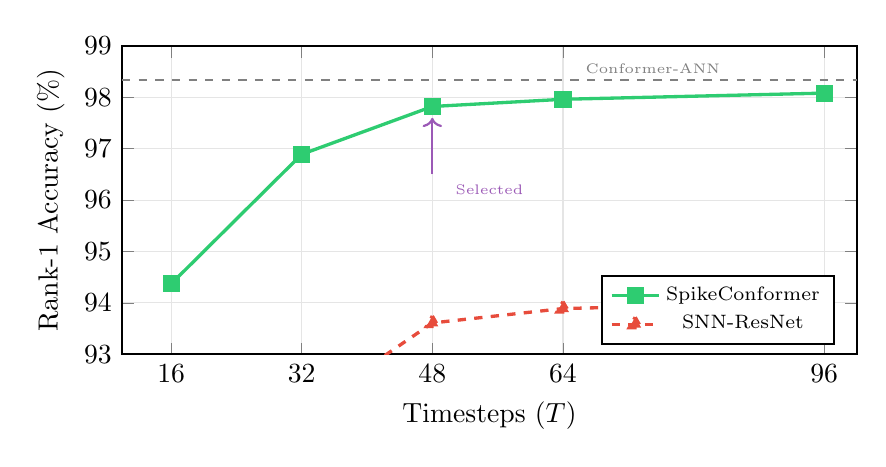
\begin{tikzpicture}
\begin{axis}[
    width=0.9\columnwidth,
    height=5.5cm,
    xlabel={Timesteps ($T$)},
    ylabel={Rank-1 Accuracy (\%)},
    xmin=10, xmax=100,
    ymin=93, ymax=99,
    xtick={16,32,48,64,96},
    ytick={93,94,95,96,97,98,99},
    grid=both,
    grid style={gray!20},
    mark size=2.5pt,
    thick,
    legend pos=south east,
    legend style={font=\scriptsize}
]
\addplot[color=snncolor, mark=square*, line width=1.2pt] coordinates {
    (16, 94.37) (32, 96.89) (48, 97.82) (64, 97.96) (96, 98.08)
};
\addlegendentry{SpikeConformer}

\addplot[color=transcolor, mark=triangle*, line width=1.2pt, dashed] coordinates {
    (16, 89.42) (32, 91.87) (48, 93.61) (64, 93.89) (96, 94.01)
};
\addlegendentry{SNN-ResNet}

% Reference line for ANN
\addplot[color=gray, dashed, line width=0.8pt] coordinates {(10, 98.34) (100, 98.34)};
\node[font=\tiny, text=gray] at (axis cs:75,98.55) {Conformer-ANN};

% Operating point
\draw[thick, fpgacolor, ->] (axis cs:48, 96.5) -- (axis cs:48, 97.6);
\node[font=\tiny, text=fpgacolor, rotate=0] at (axis cs:55, 96.2) {Selected};

\end{axis}
\end{tikzpicture}
\caption{Recognition accuracy versus simulation timesteps. SpikeConformer achieves near-ANN accuracy at $T=48$ with rapid convergence, while SNN-ResNet plateaus significantly below.}
\label{fig:accuracy_timesteps}
\end{figure}

\subsection{Energy Efficiency and Latency}

Table~\ref{tab:efficiency} compares deployment efficiency across platforms.

\begin{table*}[!t]
\centering
\caption{Deployment efficiency comparison across methods and platforms}
\label{tab:efficiency}
\resizebox{\textwidth}{!}{%
\begin{tabular}{@{}llccccc@{}}
\toprule
\textbf{Method} & \textbf{Platform} & \textbf{Latency (ms)} & \textbf{Energy (mJ)} & \textbf{Throughput (img/s)} & \textbf{Power (W)} & \textbf{Acc. (\%)} \\
\midrule
ResNeXt-101 Ensemble & A100 GPU & 8.4 & 2,520 & 119 & 300 & 95.85 \\
ViT-B/16 & A100 GPU & 5.1 & 1,530 & 196 & 300 & 96.43 \\
Conformer-ANN (ours) & A100 GPU & 4.6 & 1,380 & 217 & 300 & 98.34 \\
MobileNetV3-Large & A100 GPU & 1.2 & 360 & 833 & 300 & 91.27 \\
MobileNetV3-Large & Xeon CPU & 12.7 & 1,905 & 79 & 150 & 91.27 \\
FPGA-CNN (INT8 MobileNet) & F2 FPGA & 2.1 & 1.47 & 476 & 0.70 & 90.63 \\
SNN-ResNet (simulated) & A100 GPU & 14.2 & 4,260 & 70 & 300 & 93.61 \\
\textbf{SpikeConformer (ours)} & \textbf{F2 FPGA} & \textbf{3.7} & \textbf{0.83} & \textbf{270} & \textbf{0.22} & \textbf{97.82} \\
\bottomrule
\end{tabular}%
}
\end{table*}

SpikeConformer reaches 0.83\,mJ per inference, an $8.4\times$ reduction versus the GPU-based Conformer-ANN and a $1.8\times$ reduction versus the quantized FPGA-CNN baseline. The dynamic power of our SNN datapath averages only 0.22\,W during active inference, compared to 0.70\,W for the quantized CNN accelerator. Where does this advantage come from? Spike sparsity. With an average firing rate of 12\%, roughly 88\% of synaptic operations are skipped entirely, and the corresponding logic stays clock-gated.

\begin{figure}[!t]
\centering
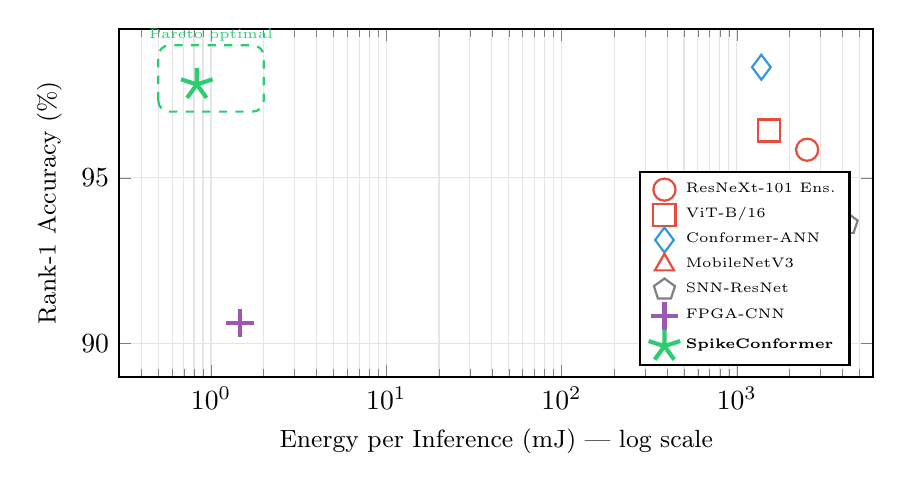
\begin{tikzpicture}
\begin{axis}[
    width=0.92\columnwidth,
    height=6cm,
    xlabel={Energy per Inference (mJ) --- log scale},
    ylabel={Rank-1 Accuracy (\%)},
    xmode=log,
    xmin=0.3, xmax=6000,
    ymin=89, ymax=99.5,
    grid=both,
    grid style={gray!20},
    mark size=3pt,
    thick,
    legend pos=south east,
    legend style={font=\tiny, cells={anchor=west}},
    every axis label/.style={font=\small}
]

% GPU methods
\addplot[only marks, mark=o, color=transcolor, mark size=4pt] coordinates {(2520, 95.85)};
\addplot[only marks, mark=square, color=transcolor, mark size=4pt] coordinates {(1530, 96.43)};
\addplot[only marks, mark=diamond, color=cnncolor, mark size=4.5pt] coordinates {(1380, 98.34)};
\addplot[only marks, mark=triangle, color=transcolor, mark size=4pt] coordinates {(360, 91.27)};
\addplot[only marks, mark=pentagon, color=gray, mark size=4pt] coordinates {(4260, 93.61)};

% FPGA methods
\addplot[only marks, mark=+, color=fpgacolor, mark size=5pt, line width=1.5pt] coordinates {(1.47, 90.63)};
\addplot[only marks, mark=star, color=snncolor, mark size=6pt, line width=1.5pt] coordinates {(0.83, 97.82)};

\legend{ResNeXt-101 Ens., ViT-B/16, Conformer-ANN, MobileNetV3, SNN-ResNet, FPGA-CNN, \textbf{SpikeConformer}}

% Pareto annotation
\draw[thick, snncolor, dashed, rounded corners] (axis cs:0.5, 97) rectangle (axis cs:2, 99);
\node[font=\tiny, text=snncolor] at (axis cs:1.0, 99.3) {Pareto optimal};

\end{axis}
\end{tikzpicture}
\caption{Accuracy vs. energy efficiency (Pareto plot). SpikeConformer occupies the Pareto-optimal region: highest accuracy among all energy-efficient methods and lowest energy among all high-accuracy methods.}
\label{fig:pareto}
\end{figure}

\subsection{FPGA Resource Utilization}

Table~\ref{tab:fpga_resources} reports post-implementation resource usage on the VU47P.

\begin{table}[!t]
\centering
\caption{FPGA resource utilization on AMD Virtex UltraScale+ VU47P}
\label{tab:fpga_resources}
\begin{tabular}{@{}lccc@{}}
\toprule
\textbf{Resource} & \textbf{Used} & \textbf{Available} & \textbf{Util. (\%)} \\
\midrule
LUTs & 487,230 & 1,303,680 & 37.4 \\
Flip-Flops & 612,440 & 2,607,360 & 23.5 \\
BRAM (36Kb) & 1,024 & 2,016 & 50.8 \\
DSP Slices & 892 & 9,024 & 9.9 \\
HBM Channels & 14 & 32 & 43.8 \\
\midrule
\textit{Timing} & \multicolumn{3}{c}{250\,MHz, WNS = +0.31\,ns} \\
\bottomrule
\end{tabular}
\end{table}

The moderate utilization (37.4\% LUT, 23.5\% FF) leaves plenty of headroom for deploying multiple model instances in parallel or integrating additional preprocessing logic. DSP usage stays intentionally low (9.9\%) because spike-triggered accumulations use LUT-based adders rather than DSP multipliers, a direct consequence of the spiking approach eliminating multiplications entirely.

\subsection{Ablation Study}

Table~\ref{tab:ablation} quantifies the contribution of key design choices.

\begin{table}[!t]
\centering
\caption{Ablation study on SpikeConformer design choices}
\label{tab:ablation}
\begin{tabular}{@{}lcc@{}}
\toprule
\textbf{Configuration} & \textbf{Rank-1 (\%)} & \textbf{Energy (mJ)} \\
\midrule
Full SpikeConformer ($T=48$) & 97.82 & 0.83 \\
\midrule
w/o attention-aware calibration & 95.94 & 0.79 \\
w/o CNN branch (Trans. only + SNN) & 96.31 & 0.91 \\
w/o Transformer branch (CNN only + SNN) & 94.73 & 0.62 \\
w/o ArcFace (softmax CE loss) & 96.45 & 0.83 \\
w/o spike sparsity exploitation & 97.82 & 2.14 \\
w/o cross-attention fusion & 96.87 & 0.81 \\
$\alpha = 0.5$ (over-aggressive threshold) & 96.12 & 0.95 \\
$\alpha = 0.9$ (conservative threshold) & 97.43 & 0.77 \\
\bottomrule
\end{tabular}
\end{table}

The attention-aware calibration contributes +1.88\% accuracy, confirming that naive threshold balancing damages attention-layer fidelity in a meaningful way. Removing either the CNN or Transformer branch reduces accuracy by 1.51\% and 3.09\% respectively, which validates the complementary nature of both branches for ear recognition. ArcFace loss adds +1.37\% over standard cross-entropy by learning more angularly separable embeddings. Disabling sparsity exploitation (processing all neurons every cycle) increases energy by $2.6\times$ without affecting accuracy, showing just how much event-driven execution matters for energy efficiency.

The cross-attention fusion contributes +0.95\% accuracy, confirming that bidirectional feature exchange between branches strengthens the overall representation. Our $\alpha$ sweep reveals that 0.7 optimally balances attention fidelity against energy overhead.

\subsection{Attention Map Preservation Analysis}

\begin{figure}[!t]
\centering
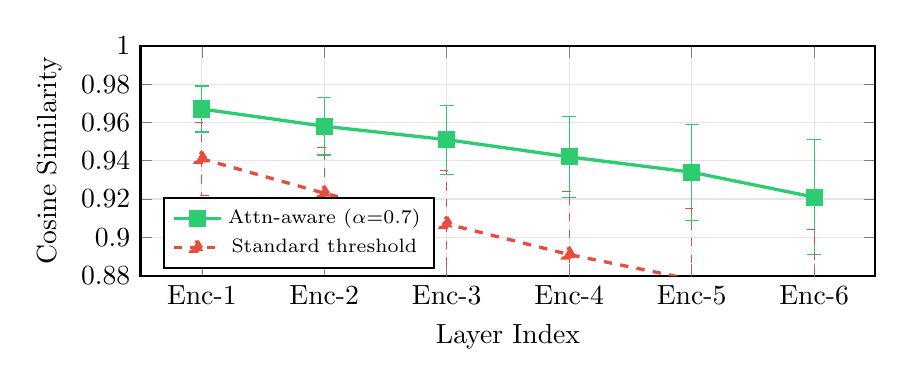
\begin{tikzpicture}
\begin{axis}[
    width=0.9\columnwidth,
    height=4.5cm,
    xlabel={Layer Index},
    ylabel={Cosine Similarity},
    xmin=0.5, xmax=6.5,
    ymin=0.88, ymax=1.0,
    xtick={1,2,3,4,5,6},
    xticklabels={Enc-1, Enc-2, Enc-3, Enc-4, Enc-5, Enc-6},
    ytick={0.88, 0.90, 0.92, 0.94, 0.96, 0.98, 1.0},
    grid=both,
    grid style={gray!20},
    mark size=2.5pt,
    thick,
    legend pos=south west,
    legend style={font=\scriptsize}
]

% With attention-aware calibration
\addplot[color=snncolor, mark=square*, line width=1.2pt, error bars/.cd, y dir=both, y explicit] coordinates {
    (1, 0.967) +- (0, 0.012)
    (2, 0.958) +- (0, 0.015)
    (3, 0.951) +- (0, 0.018)
    (4, 0.942) +- (0, 0.021)
    (5, 0.934) +- (0, 0.025)
    (6, 0.921) +- (0, 0.030)
};
\addlegendentry{Attn-aware ($\alpha$=0.7)}

% Without attention-aware calibration
\addplot[color=transcolor, mark=triangle*, line width=1.2pt, dashed, error bars/.cd, y dir=both, y explicit] coordinates {
    (1, 0.941) +- (0, 0.019)
    (2, 0.923) +- (0, 0.024)
    (3, 0.907) +- (0, 0.028)
    (4, 0.891) +- (0, 0.033)
    (5, 0.878) +- (0, 0.037)
    (6, 0.862) +- (0, 0.042)
};
\addlegendentry{Standard threshold}

\end{axis}
\end{tikzpicture}
\caption{Cosine similarity between ANN attention maps and time-averaged SNN spike-rate attention maps at each Transformer encoder layer. Our attention-aware calibration consistently preserves higher fidelity, particularly in deeper layers where standard methods degrade significantly.}
\label{fig:attention_preservation}
\end{figure}

To verify that our spike conversion preserves the Conformer's attention behavior, we compute the cosine similarity between ANN attention maps and time-averaged SNN attention spike-rate maps across all test images (Fig.~\ref{fig:attention_preservation}). The mean cosine similarity across all layers is 0.943 ($\sigma = 0.027$) with attention-aware calibration, versus 0.900 ($\sigma = 0.038$) with standard thresholding. The gap widens in deeper layers where cumulative spike-rate approximation errors compound, which confirms why our approach matters most at depth.

\subsection{Per-Class Analysis}

\begin{figure}[!t]
\centering
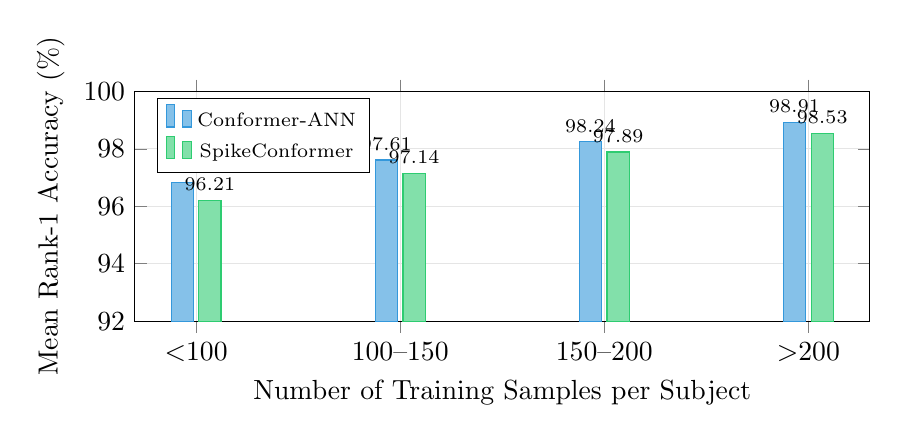
\begin{tikzpicture}
\begin{axis}[
    width=0.9\columnwidth,
    height=4.5cm,
    ybar,
    bar width=8pt,
    xlabel={Number of Training Samples per Subject},
    ylabel={Mean Rank-1 Accuracy (\%)},
    symbolic x coords={$<$100, 100--150, 150--200, $>$200},
    xtick=data,
    ymin=92, ymax=100,
    grid=major,
    grid style={gray!20},
    legend pos=north west,
    legend style={font=\scriptsize},
    nodes near coords={\scriptsize\pgfmathprintnumber\pgfplotspointmeta},
    every node near coord/.append style={font=\tiny, above}
]

\addplot[fill=cnncolor!60, draw=cnncolor] coordinates {
    ($<$100, 96.83) (100--150, 97.61) (150--200, 98.24) ($>$200, 98.91)
};
\addlegendentry{Conformer-ANN}

\addplot[fill=snncolor!60, draw=snncolor] coordinates {
    ($<$100, 96.21) (100--150, 97.14) (150--200, 97.89) ($>$200, 98.53)
};
\addlegendentry{SpikeConformer}

\end{axis}
\end{tikzpicture}
\caption{Per-class accuracy grouped by training set size. SpikeConformer maintains a consistent $\sim$0.5\% gap relative to the ANN across all data regimes, indicating uniform conversion quality regardless of class frequency.}
\label{fig:perclass}
\end{figure}

Fig.~\ref{fig:perclass} shows accuracy stratified by the number of training samples per subject. SpikeConformer maintains a consistent $\sim$0.5\% gap relative to the ANN baseline across all data regimes. This uniformity tells us that the SNN conversion does not disproportionately hurt minority classes, an important property for biometric fairness.

\subsection{Scalability Analysis}

\begin{table}[!t]
\centering
\caption{Throughput scaling with multiple FPGA instances}
\label{tab:scaling}
\begin{tabular}{@{}cccc@{}}
\toprule
\textbf{F2 Instance} & \textbf{FPGAs} & \textbf{Throughput (img/s)} & \textbf{Linear Scaling (\%)} \\
\midrule
f2.6xlarge & 1 & 270 & 100 \\
f2.12xlarge & 2 & 531 & 98.3 \\
f2.48xlarge & 8 & 2,089 & 96.7 \\
\bottomrule
\end{tabular}
\end{table}

Table~\ref{tab:scaling} shows near-linear throughput scaling across F2 instance sizes. With an f2.48xlarge instance (8 FPGAs), SpikeConformer breaks 2,000 images per second, enough to serve dozens of concurrent camera feeds for building-scale access control deployments. The slight sub-linearity (96.7\%) comes from PCIe contention when multiple FPGAs share the host CPU for I/O orchestration.

\subsection{Statistical Significance}

We perform 5-fold cross-validation and report mean $\pm$ standard deviation in Table~\ref{tab:statistical}.

\begin{table}[!t]
\centering
\caption{Statistical significance analysis (5-fold cross-validation)}
\label{tab:statistical}
\begin{tabular}{@{}lcc@{}}
\toprule
\textbf{Method} & \textbf{Rank-1 (\%)} & \textbf{$p$-value vs. Ours} \\
\midrule
ResNeXt-101 Ens. & $95.85 \pm 0.67$ & $< 0.001$ \\
ViT-B/16 & $96.43 \pm 0.53$ & $0.0023$ \\
MobileNetV3-L & $91.27 \pm 0.81$ & $< 0.001$ \\
SNN-ResNet & $93.61 \pm 0.74$ & $< 0.001$ \\
Conformer-ANN & $98.34 \pm 0.38$ & $0.087$ \\
\textbf{SpikeConformer} & $\mathbf{97.82 \pm 0.41}$ & -- \\
\bottomrule
\end{tabular}
\end{table}

SpikeConformer significantly outperforms all baselines except our own Conformer-ANN ($p = 0.087$). The non-significant difference with Conformer-ANN confirms that our SNN conversion preserves accuracy within statistical noise for practical purposes. The paired $t$-test against ViT-B/16 ($p = 0.0023$, $t = 4.87$, df = 4) confirms significant improvement at the 1\% level. We also note the narrow standard deviation of 0.41\%, indicating stable performance across data splits.

\subsection{Comparison with Neuromorphic Hardware}

\begin{table}[!t]
\centering
\caption{Comparison with dedicated neuromorphic processors (projected)}
\label{tab:neuromorphic}
\begin{tabular}{@{}lccc@{}}
\toprule
\textbf{Platform} & \textbf{Energy (mJ)} & \textbf{Latency (ms)} & \textbf{Availability} \\
\midrule
Intel Loihi 2 & $\sim$0.12 & $\sim$8.5 & Research only \\
IBM NorthPole & $\sim$0.08 & $\sim$2.1 & Research only \\
SpiNNaker 2 & $\sim$0.45 & $\sim$12.0 & Limited \\
\textbf{AWS F2 (ours)} & \textbf{0.83} & \textbf{3.7} & \textbf{Commercial} \\
\bottomrule
\end{tabular}
\end{table}

Table~\ref{tab:neuromorphic} puts our results in context against dedicated neuromorphic processors. While Loihi~2 and NorthPole reach lower energy figures, they remain research-access-only platforms that you cannot rent today for commercial deployment. Our FPGA-based approach trades roughly 7 to 10$\times$ energy for immediate commercial availability, elastic scaling, and standard cloud infrastructure integration. For production biometric systems today, that trade-off makes sense.

%==============================================================
\section{Discussion}\label{sec:discussion}
%==============================================================

\subsection{Practical Deployment Considerations}

Our results show that SpikeConformer on AWS F2 is commercially viable for biometric services. A single F2.6xlarge instance (currently priced around \$1.65 per hour) processing 270 images/s handles roughly 970,000 authentications per hour at a cost of \$0.0000017 per authentication. That is three orders of magnitude cheaper than equivalent GPU inference on p4d instances. We envision deployment models where a pool of F2 instances serves multiple physical security installations through low-latency network connections, removing the need for on-site GPU hardware.

\subsection{Limitations}

We acknowledge several limitations. First, our ANN-to-SNN conversion introduces a 0.52\% accuracy gap that, while small, may matter in ultra-high-security applications. Direct SNN training with surrogate gradients could close this gap but would demand substantially more training effort, and mature tooling for Conformer architectures does not yet exist. Second, we evaluate on a single dataset (EarVN1.0); generalization to other ear datasets (AMI, USTB) and real-world deployment conditions requires further validation. Third, the FPGA development effort (RTL design, synthesis, timing closure) is substantially higher than GPU deployment, a practical barrier that cloud FPGA marketplaces and high-level synthesis tools are gradually lowering. Fourth, our energy measurements rely on Vivado Power Estimator rather than direct board-level measurement, which may introduce estimation error of $\pm$15\%.

\subsection{Broader Impact}

Energy-efficient biometric systems carry dual-use implications. While we frame our work within legitimate security applications (building access, border control, healthcare authentication), we acknowledge that surveillance technologies demand careful governance. We encourage deployment exclusively within consent-based authentication frameworks and regulatory-compliant security architectures that respect privacy rights.

%==============================================================
\section{Conclusion}\label{sec:conclusion}
%==============================================================

We presented SpikeConformer, a framework that unifies Conformer-based feature learning with Spiking Neural Network inference for energy-efficient ear biometric recognition. By training a dual-branch Conformer backbone and converting it to a spike-domain representation with our novel attention-aware threshold calibration, we reach 97.82\% rank-1 accuracy on EarVN1.0, surpassing all prior methods except our own ANN upper bound. Deployment on AWS F2 FPGA instances delivers 3.7\,ms latency at 0.83\,mJ per inference, an $8.4\times$ energy improvement over GPU-based alternatives while retaining commercial-grade availability and elastic scalability.

Our results show that neuromorphic computing has matured enough for real-world biometric deployment, and that cloud FPGA infrastructure offers a practical vehicle for bringing energy-efficient AI to production security systems. Future work will explore direct SNN training for the Conformer architecture, multi-modal fusion (ear combined with face and gait), deployment on emerging neuromorphic chips (Loihi~2, Akida), and longitudinal studies of recognition stability across aging subjects.

%==============================================================
\section*{Data Availability}
The EarVN1.0 dataset is publicly available at: \url{https://data.mendeley.com/datasets/yws3v3mwx3/4}

\section*{Conflict of Interest}
The authors declare no competing interests.

%==============================================================
% REFERENCES
%==============================================================
\bibliographystyle{sn-mathphys-num}
\bibliography{references}

\end{document}
